\documentclass{article}
\usepackage{tikz}
\usepackage{pdfpages}
\usepackage{parskip}
\usepackage{amsmath}
\usepackage[margin=.6in]{geometry}

\begin{document}
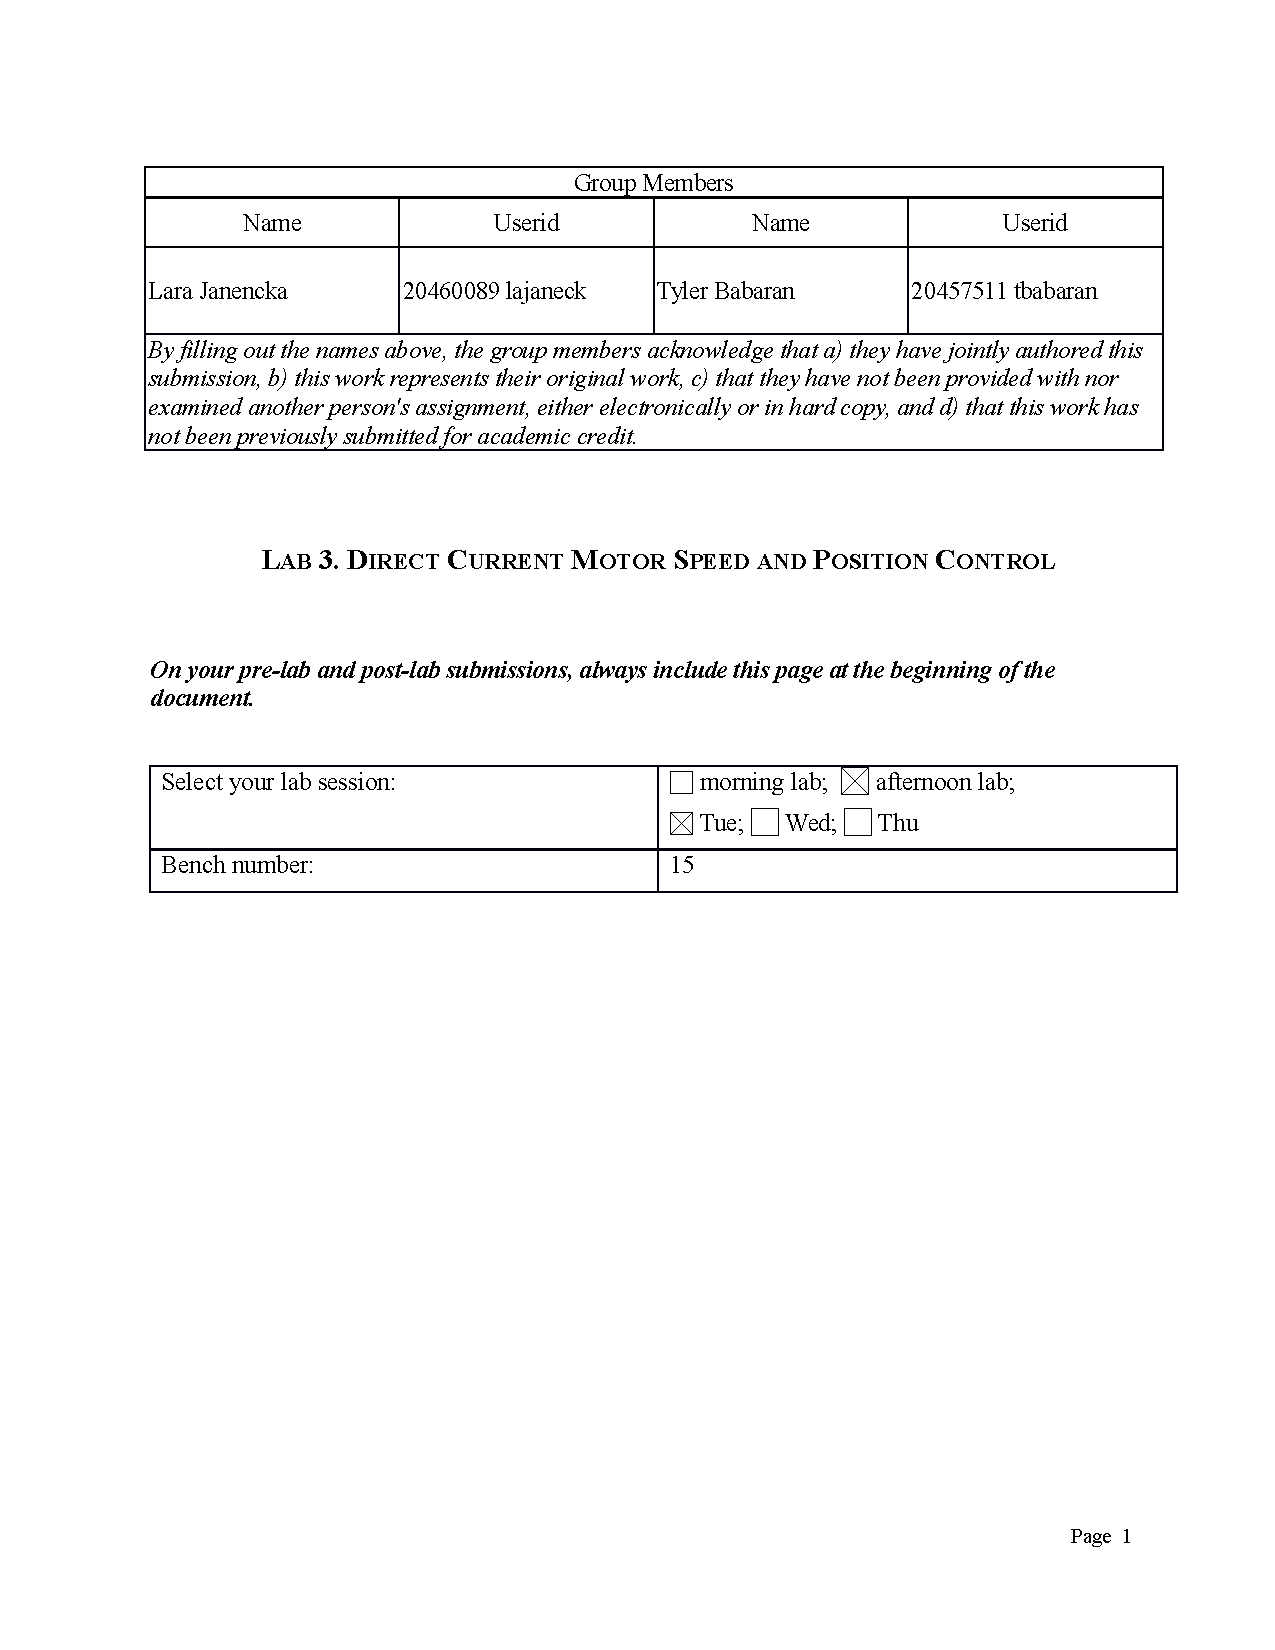
\includepdf[pages={1}]{page1.pdf}

\section*{5.1.1} % (fold)
\label{sec:5_1_1}


\begin{table}[!htbp]
\centering
    \begin{tabular}{|c|c|c|c|c|c|}
        \hline
         & \textbf{Angle (deg)} & V & $V_M$ & $V_M$/V & $V_T$ \\
         \hline
         \textbf{Dead-Zone} & 227 & 1.6 & 4.77 & 2.98 & 0.9\\
         \hline
         \textbf{Saturation} & 3.16 & 3.95 & 11.75 & 2.97 & 10.44\\
        \hline
    \end{tabular}
    \caption{Dead zone and saturation measurements}
\end{table}

\textbf{Saturation Explanation}
At some point the force that we apply is equally matched by the friction that the system pushes back with. This results in acceleration dropping to 0 and the velocity plateauing.
% section 5_1_1 (end)

\section*{5.1.2} % (fold)
\label{sec:5_1_2}

\begin{align*}
    V_M &= VK_a\\
    10 &= 3.36 \times K_a\\
    K_a &= 2.98\\
\end{align*}

Since we took our measurements at steady state we can assume that they are the values at $t = \infty$ and use the final value theorem.
\begin{align*}
    V_T &= \lim_{t\to \infty} V_T\\
        &= \lim_{s\to 0} V_M \times \frac{K}{\tau_m s + 1}\\
        &= V_M \times K\\
    K &= \frac{V_T}{V_M}\\
         &= \frac{8.2}{10}\\
         &= 0.82\\
\end{align*}

\begin{table}[!htbp]
\centering
    \begin{tabular}{|c|c|c|c|c|}
        \hline
        \textbf{Number of Rotations} & \textbf{Duration} & $V_{SmallDisk}$ & w(rot/s) & w(rot/min) \\
        \hline
        10 & 26 & 0.38 & - & -\\
        \hline
        10 & 26.07 & 0.38 & - & -\\
        \hline
        10 & 26.18 & 0.38 & - & - \\
        \hline
        - & - & 0.38 & 24.32 & 1459.2\\
        \hline
    \end{tabular}
    \caption{Experimental data for angular speed}
\end{table}

\begin{align*}
    \omega \times K_{tach}&= V_T\\
    K_{tach} &= \frac{V_T}{\omega}\\
        &= \frac{8.2}{1.4592}\\
        & = 5.62
\end{align*}
Our calculated is within 15\% of 6V so we meet tolerance amounts.

\begin{align*}
    \omega &= V_M \times K_m\\
    K_M &= \frac{\omega}{V_M}\\
        &= \frac{1.4592}{10}\\
        &= 0.14592
\end{align*}

\begin{figure}[!htbp]
\centering
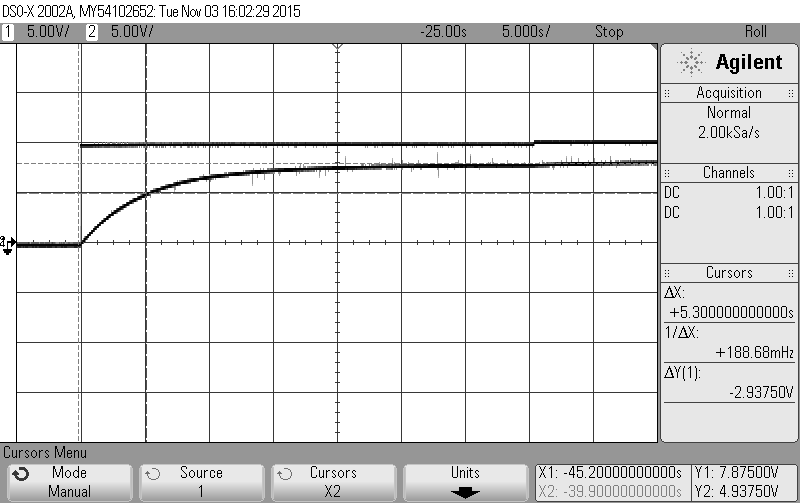
\includegraphics[width=7in]{step_response_5_2.png}
\caption{Step response of step input 1-10}
\end{figure}


\begin{table}[!htbp]
\centering
    \begin{tabular}{|c|c|c|}
        \hline
        $V_M$ & $V_{TSS}$ & $\tau_m$ \\
        \hline
        10 & 7.88 & 5.3\\
        \hline
    \end{tabular}
    \caption{Motor time-constant measurement}
\end{table}

\textbf{Experimental method for finding poles} We know that for a standard first order system as $\tau$ tends to 0 the pole will tend to $-\infty$. Using this we can muck with settings on the system an watch how $\tau$ moves. From this we can attempt to calculate the location of the pole.


\begin{table}[!htbp]
\centering
    \begin{tabular}{|c|c|c|c|c|}
        \hline
        $K_p$ & V & $V_{TSS}$ & $\tau_{cl}$ & $e_{ss}$\\
        \hline
        1 &  1 & 0.7 &  1.2 & 30\\
        \hline
        2  & 1 & 0.81 &     0.7 & 19\\
        \hline
        4  & 1 & 0.96 &     0.4 & 4\\
        \hline
    \end{tabular}
    \caption{Motor speed control data for Kp=variable}
\end{table}
\begin{figure}[!htbp]
\centering
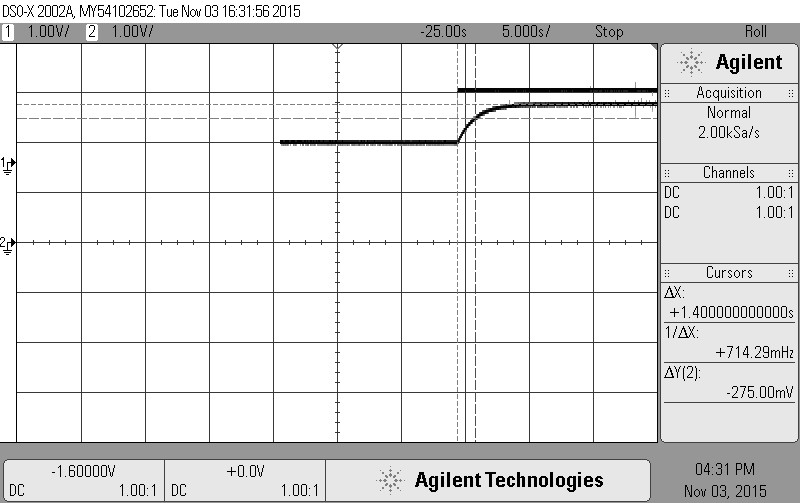
\includegraphics[width=7in]{step_response_kp1_5_2.jpg}
\caption{Step response of step input 2-3}
\end{figure}

As the gain increased proportionally it decreased the steady state error making the performance of our system closer match the input. This fits with control theory by looking at the final value theorem. We can see from our prelab that the steady state error signal is inversely related to K so as K tends to infinity the error signal will tend to 0.

\begin{table}[!htbp]
\centering
    \begin{tabular}{|c|c|c|c|c|c|c|}
        \hline
        $K_p$ & V & $V_{Omax}$ & $C_{OSS}$ & OS & $T_p$ & $e_{ss}$\\
        \hline
        3   & 3     & 4.15     & 3.1   & 38 & 4.12 & 3\\
        \hline
        4   & 3     & 3.8      & 2.8    & 27 & 3.92 & 7\\
        \hline
        5   & 3     & 3.65     & 2.58   & 27 & 3.73 & 14\\
        \hline
    \end{tabular}
    \caption{Motor position control data for Kp=variable}
\end{table}
\begin{figure}[!htbp]
\centering
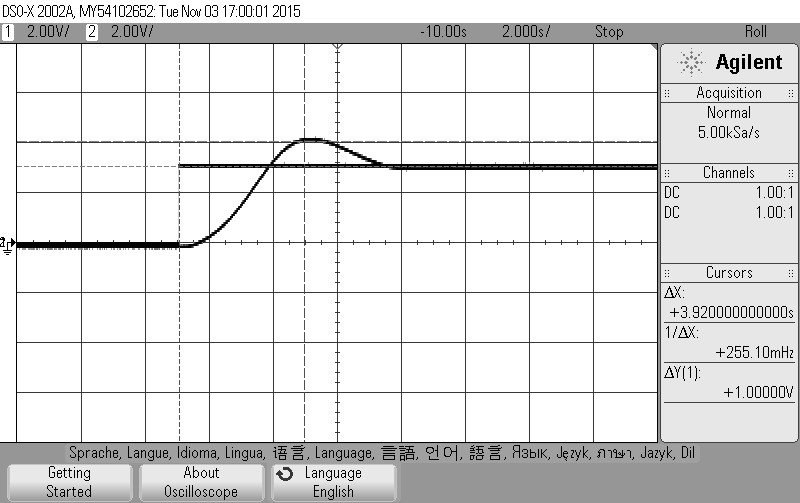
\includegraphics[width=7in]{step_response_kp1_second_5_2.jpg}
\caption{Step response of step input 0-3}
\end{figure}

As gain increases the overshoot decreases we fits with control theory as in our prelab we found that $\zeta$ is inversly proportional to K and that overshoot is proportional to $\zeta$. This means that as K tends to infinity the overshoot tends to zero. As gain increased we found that the steady state error increased as well. This does not fit with control theory as we saw in our prelab that the steady state error should not at all be related to K as it is equal to zero. This could be due to error in reading measurements or inaccuracies in setting values. It is also likely due to the fact that we are dealing with a non-ideal system where friction and other forces may effect results.

% section 5_1_2 (end)

\end{document}
